\documentclass[a4paper,10pt]{article}

% Packages
\usepackage{microtype}
\usepackage[english]{babel}           
\usepackage[latin1]{inputenc}       	% speciale karakters
\usepackage{graphicx} 				% figuren
\usepackage[hyphens]{url}
\usepackage{hyperref}
\usepackage{subfigure}
\usepackage{amssymb}
\usepackage{amsmath}
\usepackage{graphicx}
\usepackage[font=small,format=plain,labelfont=bf,up,textfont=it,up]{caption}
\usepackage{float}
\usepackage{multirow,tabularx}
\usepackage[bottom]{footmisc}
\usepackage[T1]{fontenc}
\usepackage{lmodern}
\usepackage{lastpage}
\usepackage{fancyhdr}
\usepackage{listings}
\usepackage{enumitem}
\usepackage{hvfloat}
\usepackage{color}

\newcolumntype{Y}{>{\centering\arraybackslash}X}

\definecolor{mygreen}{rgb}{0,0.6,0}
\definecolor{mygray}{rgb}{0.5,0.5,0.5}
\definecolor{mymauve}{rgb}{0.58,0,0.82}

\lstset{ %
	backgroundcolor=\color{white},   % choose the background color; you must add \usepackage{color} or \usepackage{xcolor}
	basicstyle=\footnotesize,        % the size of the fonts that are used for the code
	breakatwhitespace=false,         % sets if automatic breaks should only happen at whitespace
	breaklines=true,                 % sets automatic line breaking
	captionpos=b,                    % sets the caption-position to bottom
	commentstyle=\color{mygreen},    % comment style
	deletekeywords={},            % if you want to delete keywords from the given language
	escapeinside={\%*}{*)},          % if you want to add LaTeX within your code
	extendedchars=true,              % lets you use non-ASCII characters; for 8-bits encodings only, does not work with UTF-8
	frame=single,                    % adds a frame around the code
	keepspaces=true,                 % keeps spaces in text, useful for keeping indentation of code (possibly needs columns=flexible)
	keywordstyle=\color{blue},       % keyword style
	language=Octave,                 % the language of the code
	morekeywords={*,...},            % if you want to add more keywords to the set
	numbers=left,                    % where to put the line-numbers; possible values are (none, left, right)
	numbersep=5pt,                   % how far the line-numbers are from the code
	numberstyle=\tiny\color{mygray}, % the style that is used for the line-numbers
	rulecolor=\color{black},         % if not set, the frame-color may be changed on line-breaks within not-black text (e.g. comments (green here))
	showspaces=false,                % show spaces everywhere adding particular underscores; it overrides 'showstringspaces'
	showstringspaces=false,          % underline spaces within strings only
	showtabs=false,                  % show tabs within strings adding particular underscores
	stepnumber=1,                    % the step between two line-numbers. If it's 1, each line will be numbered
	stringstyle=\color{mymauve},     % string literal style
	tabsize=2,                       % sets default tabsize to 2 spaces
	title=\lstname                   % show the filename of files included with \lstinputlisting; also try caption instead of title
}

% Optional settings
\setlength{\hoffset}{-1.2cm}   
\addtolength{\textwidth}{2.0cm}
\setlength{\voffset}{-1.2cm}
\addtolength{\textheight}{2.0cm}

\setcounter{tocdepth}{3}
\setcounter{secnumdepth}{3}
\def\thesection{\arabic{section}}

\pagestyle{fancy}
\lhead{Group 40}
\rhead{Report: Error Correction in Digital Video}

\setlist[itemize]{noitemsep, topsep=0pt, leftmargin=*}

\begin{document}
\begin{titlepage}

\fontsize{12pt}{14pt}
\selectfont

\begin{center}


\includegraphics[height=3cm]{includes/images/UGent}

\vspace{0.5cm}

Faculty of Engineering\\
Master of Science in Computer Science\\

\vspace{4.0cm}

\fontseries{bx}
\fontsize{17.28pt}{21pt}
\selectfont

\textbf{DESIGN OF MULTIMEDIA APPLICATIONS} \\
\vspace{40pt}

\hrule
\vspace{20pt}
\textsc{Group 40}\\
\vspace{10pt}
\textbf{Report: Error Correction in Digital Video}\\
\vspace{20pt}
\hrule

\vspace{25pt}

\fontseries{m}
\fontsize{12pt}{14pt}
\selectfont

\vspace{5.0cm}

\fontseries{m}
\fontsize{12pt}{14pt}
\selectfont

\hspace{0.5cm} Group 40
\textbf{ 
	\hfill\textsc{Naessens} Tom\\
	\hfill\textsc{Van Den Bossche} Pieter\\
	\hfill\textsc{Wijnant} Joris\\
}
\end{center}
\end{titlepage}

\section{Implementation of method 5}
This detection algorithm is made to detect both hard (abrupt changes) and soft (fades) cut. It is based on the work of Zuzana Cernekova, IoannisPitas and Christophoros Nikou\cite{1564125}. According to their published work, the algorithm can detect both fades and abrupt cuts with high accuracy.

The method for shot boundary detection relies on the mutual information (MI) and the joint entropy (JE) between the frames. This mutual information for detecting hard cuts and the joint entropy for detecting soft cuts. To calculate the mutual information en joint entropy, a transition matrix and histograms are needed. These transitionmatrix and histograms are created for every component of the pixel (Red, Green and Blue). 

The transition matrix for the red component indicates how many pixels with a red value of x will take a red value of y in the next frame. Similarly for the Green and Blue components. To prevent the use off ridiculous high thresholds, the calculated values are normalised. This normalisation will be based on the mutual information and joint entropy of the change from a full black frame to a full white frame. Because in this case, both frames have nothing in common, thus the resulting values will be maximized.

Our implementation of this detection algorithm is as follows:
\begin{lstlisting}
doShotDetection(frame){

  rbgHistogram = calculateRBGHistogram(frame);

  if( not_first_frame) {

    RBGTransition = calculateRBGTransition(prevframe, frame);
    MI = calculateMutualInformation(RBGTransition, prevHistogram, rbgHistogram);
    JE = calculateJointEntropy(TBGTransition);

    if( hardCutDetected(MI) or softCutDetected(JE) ) {

      shotDetected(frame);

    }
  }

  prevHistogram = rbgHistogram;
}
\end{lstlisting}

\section{Used parameters and explanatory notes}
\subsection{Method 1. Pixel Difference Shot Detection}
Pixel difference takes two arguments, being two thresholds, as described in the assignment, corresponding to $\delta_2$ and $\delta_3$. 

The \textbf{first threshold} is the amount of difference a pixel is allowed to have from its corresponding pixel in the previous frame, before it is count as a significant different pixel. We compare each R, G and B value with these values of the pixel in the previous frame. The maximum difference is when we compare a black pixel to a white pixel. This has a difference of 3 times 255, resulting in 765. The minimum value is when we compare a pixel to an exact
same corresponding pixel, resulting in 0.

The \textbf{second threshold} is a double and corresponds with the amount of pixels in the current frame which are significantly different to the total number of pixels in the frame. When no pixels are different, this results in 0 and when all pixels are different, this results in 1.

\subsection{Method 2. Motion Estimation Comparison }
The Motion Estimation Comparison takes three arguments. The first one is the \textbf{size of the macro blocks} used to detect motion. This size is used for both the width and the height. The second one is the \textbf{size of the search window}. This window is used to find the best matching block in the previous frame.The value for search window is defined as the distance in pixels between the boundary of the macro block and the search window if they are both centred in the same point. Lastly a \textbf{threshold} is expected.

The threshold will be compared with a value identifying the best matching blocks. This value is calculated similar as the method in the first method by comparing each pixel in the macro block and the matching pixel in the block of the previous frame. This value is normalised to a value between 0 en 10.

\subsection{Method 3. Global Histogram Comparison}
The Global Histogram Comparison takes 2 arguments, a threshold and the number of bins.

The \textbf{threshold} is used to determine if the current frame is a new shot or not. If the cumulative absolute difference between frame(N).bin(i) and frame(N-1).bin(i), over every i, is greater than the given threshold for the R, G and B histogram, then we conclude that frame N is a new shot.
\textit{Important note: in the first version of the code, as it was sent to the assistance there was a mistake in the normalisation process! This made the difference sums inversely proportional to the number of bins. This has been fixed in a second version of the code and the values for threshold in this document use the new version of the code, where the threshold should be in the [0,100] range.}

The number of \textbf{bins} determines in how many chunks a histogram for R, G and B are divided in. A normal histogram would consist out of 256 values, but for performance reasons we can easily group certain values together, forming bins. For example we could group every 8 values together, resulting in 32 bins per histogram.

\subsection{Method 4. Local Histogram Comparison}
The Local Histogram Comparison takes 3 arguments, a threshold, the number of bins and a region-size.

Local Histogram Comparison, opposed to the Global variant, compares histograms on a local level. Instead of creating histograms of the entire frame, it creates multiple histograms per frame that contain information about predefined blocks inside the frame. The size of these blocks are determined by the \textbf{region size} parameter. The exact dimensions of the blocks are proportional to the dimensions of the frame, this gets calculated during the initialisation of the Local Histogram Comparison class. Because dividing the frame in 9 blocks seems to be the recommended amount, the value 0 can be used as the region size, this will result in the usage 9 blocks.

The \textbf{threshold} is used to determine if the current frame is a new shot or not. If the cumulative absolute difference between frame(N).block(j).bin(i) and frame(N-1).block(j).bin(i), over every i and j, is greater than the given threshold for the R, G and B histogram, then we
conclude that frame N is a new shot.

The number of \textbf{bins} determines in how many chunks a histogram for R, G and B are divided in. A normal histogram would consist out of 256 values, but for performance reasons we can easily group certain values together, forming bins. For example we could group every 8 values together, resulting in 32 bins per histogram.
\textit{Important note: in the first version of the code, as it was sent to the assistance there was a mistake in the normalisation process! This made the difference sums inversely proportional to the number of bins. This has been fixed in a second version of the code and the values for threshold in this document use the new version of the code, where the threshold should be in the [0,100] range. The changed files have been added to the zip.}

\subsection{Method 5. Generalised Detection}
This algorithm takes two parameters, a \textbf{threshold for the soft cuts} and a \textbf{threshold for the hard cuts}.
The one for the hard cuts will be compared with the calculated mutual information between two following frames. The other one for the soft cuts will be compared with the joint entropy.

\subsection{Parameter overview}
\begin{tabularx}{\textwidth}{|*{4}{Y|}}
	\hline
	\textbf{Name}			& \textbf{Type}			& \textbf{Total}		& \textbf{Useful range}			\\
	\hline
	\hline
	\hline
	\multicolumn{4}{|c|}{\textbf{1. Pixel Difference}}\\
	\hline
	\hline
	Threshold 1		& int 		& 0 -- 765	 			& 100 -- 175\\
	\hline
	Threshold 2 		& double 	& 0.0 -- 1.0			& 0.3 -- 0.55 \\
	\hline
	\hline
	\multicolumn{4}{|c|}{\textbf{2. Motion estimated}}\\
	\hline
	\hline
	Threshold			& int 	&	0 -- 10				& 2 -- 4\\
	\hline
	Block Size 			& int 	&	1 -- 100			& 16 -- 16\\
	\hline
	Search Window Size & int	& 0 -- 100				 & 16 -- 16\\
	\hline
	\hline
	\multicolumn{4}{|c|}{\textbf{3. Global histogram}}\\
	\hline
	\hline
	Threshold	& int	& 0 -- 100		  & 0 - 30\\
	\hline
	\# Bins 	& int	& 1 -- 256			& 1 -- 256 \\
	\hline
	\hline
	\multicolumn{4}{|c|}{\textbf{4. Local histogram}}\\
	\hline
	\hline
	Threshold	& int	& 0 -- 100		  & 0 - 30 \\
	\hline
	\# Bins 	& int	& 1 -- 256		  & 1 -- 256 \\
	\hline
	Region size & int	& 0 - res frame	  & 0.25 - res frame\\
	\hline
	\hline
	\multicolumn{4}{|c|}{\textbf{5. Generalised}}\\
	\hline
	\hline
	Threshold 1	& double	& 0.0 -- 1000.0		 & 400 -- 600\\
	\hline
	Threshold 2 	& double	& 0.0 -- 1.0		 & 0.8 -- 0.95 \\
	\hline
\end{tabularx}

\section{Comparative discussion of the precision and recall values}
When looking at all the results; we notice a similar trend. If we want more recall, we lose precision. This means that we find more shots, but we also find more false shots.


\section{Comparative discussion of the computational complexity of each video detection method}
\textit{Disclaimer: These tests were performed on a Dell 3500 with an Intel i3 M 350 processor, clocked at 2.27GHz. with 4 gigabytes of ram. The timing results of the optimal parameters can be seen in table \ref{bestparams} on page \pageref{bestparams}.}

\paragraph{Pixel Difference SD} This method has very low complexity. It iterates over every frame once and iterates over all the pixels in that frame. Thus, how bigger the frame and how longer the video, how longer this algorithm takes. This means that the algorithm always has the same execution time for the same video, independent from the parameters.

\paragraph{Motion Estimation SD} Motion estimation is a very complex method. It is dependent on all its parameters except of the threshold. The bigger the search window, the longer it takes to extract shots. The smaller the block size, the more comparisons have to be made and the more block sizes have to be searched in the search window. This method is computationally the heaviest method.  

\paragraph{Global Histogram SD} This method has almost the same complexity as pixel difference. It also runs over the frames and all the pixels in a frame, but has to make a little less calculations. Because of this, it is a bit faster than pixel difference SD.

\paragraph{Local Histogram SD} Local histogram has almost the same complexity as the previous method, but is a tiny bit slower then global histogram SD as a little bit more calculations have to be made.

\paragraph{Generalized SD} Our generalized SD method also runs once over all the frames and all the pixels, but it does some more comparisons on the side. For example; the entropy is calculated after every frame. In conclusion, this method takes a bit longer then the other methods that run over the frames and pixels.


\section{Benchmark results}
\textit{Disclaimer: Bigger versions of the diagram have been included in the appendix, and as well as a pdf file in the zip.}

The comparative curves for individual video sequences can be found on \ref{jedi} on page \pageref{jedi} (Return of the Jedi), \ref{csi} on pageref \pageref{csi} (CSI) and \ref{ywy} on page \pageref{ywy} (Youth without Youth). A comparative table of optimal parameter values can be found below.

\begin{figure}[ht!]
	\centering
	\includegraphics[width=100mm]{includes/images/jedi.pdf}
	\caption{ROC diagram for the Return of the Jedi video}
	\label{jedi}
\end{figure}


\begin{figure}[ht!]
	\centering
	\includegraphics[width=100mm]{includes/images/CSI.pdf}
	\caption{ROC diagram for the CSI video}
	\label{csi}
\end{figure}


\begin{figure}[ht!]
	\centering
	\includegraphics[width=100mm]{includes/images/YWY.pdf}
	\caption{ROC diagram for the Youth without Youth video}
	\label{ywy}
\end{figure}

\begin{table}
    \begin{tabular}{|l|l|r||l|l|l|l|}
    	\hline
    	~                & \textbf{Parameters}                                     & \textbf{Video}      & \textbf{Recall}             & \textbf{Prec.} & \textbf{F1} & \textbf{Time} \\ \hline
    	
    	\textbf{Method 1} & \parbox{30mm}{\begin{itemize}\item Threshold 1: 150\item Threshold 2: 0.4\end{itemize}}                    & \parbox{10mm}{Jedi \\ CSI \\ YWY}  &  \parbox{10mm}{0.67\\ 0.82\\ 0.21} & \parbox{10mm}{0.79\\ 0.84\\ 1} & \parbox{10mm}{0.72\\ 0.83\\ 0.35} & \parbox{20mm}{15636\\ 334082\\ 29493} \\ \hline
    	
    	\textbf{Method 2}  & \parbox{30mm}{\begin{itemize}\item Threshold: 3 \item Block Size: 16\item SW Size: 16\end{itemize}}  & \parbox{10mm}{Jedi \\ CSI \\ YWY}  &  \parbox{10mm}{0.29\\ 0.49\\ .15} & \parbox{10mm}{0.82\\ 0.86\\ 1} & \parbox{10mm}{0.21\\ 0.63\\ 0.26} & \parbox{20mm}{188239\\ 2109363\\ 316124} \\ \hline
    	
    	\textbf{Method 3}  &\parbox{30mm}{\begin{itemize}\item Threshold: 50 \item \# Bins: 256 \end{itemize}}                         & \parbox{10mm}{Jedi \\ CSI \\ YWY}  &  \parbox{10mm}{0.65\\ 0.80\\ 0.74} & \parbox{10mm}{0.8\\ 0.46\\ 0.31} & \parbox{10mm}{0.72\\ 0.59\\ 0.44} & \parbox{20mm}{11074\\ 236412\\ 19624} \\ \hline
    	
    	\textbf{Method 4}   & \parbox{30mm}{\begin{itemize}\item Threshold: 8\item \# Bins: 128\item Region size: 0\end{itemize}}            & \parbox{10mm}{Jedi \\ CSI \\ YWY}  &  \parbox{10mm}{0.82\\ 0.94\\ 0.74} & \parbox{10mm}{0.85\\ 0.49\\ 0.41} & \parbox{10mm}{0.83\\ 0.64\\ 0.53} & \parbox{20mm}{11498\\ 213416\\ 19170} \\ \hline
    	
    	\textbf{Method 5}       & \parbox{30mm}{\begin{itemize}\item Threshold 1: 500 \item Threshold 2: 0.92\end{itemize}}                   & \parbox{10mm}{Jedi \\ CSI \\ YWY}  &  \parbox{10mm}{0.67\\ 0.73\\ 0.29} & \parbox{10mm}{0.94\\ 0.90\\ 0.82} & \parbox{10mm}{0.39\\ 0.80\\ 0.39} & \parbox{20mm}{41177\\ 626488\\ 46838} \\ \hline
    \end{tabular}
    \caption{Best parameters with time}
    \label{bestparams}
\end{table}

\section{General discussion of differences between the video shot detection}
Motion estimation is obviously the worst method judged by the ROC curves and the timing measurements. This is followed by the fifth method, the general shot detection. Local and global histogram SD and pixel difference SD are obviously the fastest methods, with local histogram performing the best of all.

\section{Questions}
\paragraph{Can a clear winner be found for all different video shot detection methods and parameters settings?} Judging by the ROC curves and the timing information local histogram SD is a clear winner.

\paragraph{For the clear winner found, or for the video shot detection method that you would use in practise: How would you further improve this method in terms of precision and in terms of processing speed?} At the moment, this algorithm is not concurrently implemented. If we write the code for a GPU and a introduce multi threading, this method would be a lot faster.

\paragraph{What is the obvious shortcoming in practical scenarios, that the different video shot detection methods have in common, and how would you deal with this?}
When assembling the ROC graphs, we noticed that for 3 different frames, the same parameters can lead to enormous differences in F1 value for the same method. One shot detection method also provides much better results for some type of videos. This creates a huge diversity in the different input parameters, making it never clear what parameters to use without having to experiment beforehand. This could be partly dealt with by normalising the used parameters, but even then, this can not be prevented completely because of the inherent differences in video.

The biggest shortcoming of shot annotation on the other hand is explained in the last paragraph of the last question.

\paragraph{Given a video sequence produced by a wearable device like Google Glass, what issues does a method for video shot detection need to overcome?}
The first issue is that this is a constant stream of frames that can not really be split into shots. However, we can define shots differently here such as ``video taken on a specific place (room, ...)''. This can be combined with motion information achieved by for example a GPS tracker to annotate shots. 

\paragraph{Why is it important to add metadata to video content?}
Today on the web, there is a lot of video content. Unlike with textual data, we can't just use \texttt{Ctrl-F} to find a specific part we're looking for.
Metadata solves this problem by assigning tags and annotations to shots and videos so we can search this metadata and find the videos or shots we need.

\paragraph{Given the annotation and retrieval functionality of the application written, what are some of the problems that you foresee when you would deploy this application in the real world?}
The biggest problem we see is language. People can annotate different shots in the language and style they want. If we annotate a video in Dutch, someone who speaks Italian will probably not find the shots we have annotated when he searches in his own language. It would be better to annotate shots using some sort of ontology, such as OWL, to annotate videos.

Another problem is the need to manually annotate the different shots. The complete process of shot annotation would include that a video can automatically be split into shots and also automatically annotated. Up until this point, this last piece is missing.

\newpage
\section*{Attachments}
\begin{figure}[ht!]
	\centering
	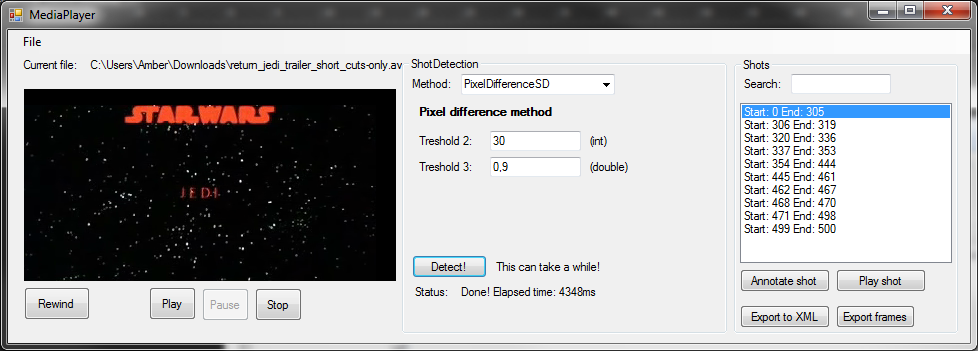
\includegraphics[width=150mm]{includes/images/mediaplayer.png}
	\caption{Our media player}
\end{figure}

\begin{figure}[ht!]
	\centering
	\includegraphics[angle=90]{includes/images/jedi.pdf}
	\caption{ROC diagram for the Return of the Jedi video}
\end{figure}


\begin{figure}[ht!]
	\centering
	\includegraphics[angle=90]{includes/images/CSI.pdf}
	\caption{ROC diagram for the CSI video}
\end{figure}


\begin{figure}[ht!]
	\centering
	\includegraphics[angle=90]{includes/images/YWY.pdf}
	\caption{ROC diagram for the Youth without Youth video}
\end{figure}

\bibliographystyle{plain}
\bibliography{references}

\end{document}
